\documentclass{article}
\usepackage{amsbsy,amscd,amsfonts,amsgen,amsmath,amsopn,amssymb,amstext,amsthm,amsxtra}
\usepackage{graphicx}
\usepackage{hyperref}
\usepackage{multirow}
\usepackage{verbatim}
\addtolength{\textwidth}{1.5in}
\addtolength{\hoffset}{-.75in}
\addtolength{\textheight}{1in}
\addtolength{\voffset}{-1in}

% Alter some LaTeX defaults for better treatment of figures:
    % See p.105 of "TeX Unbound" for suggested values.
    % See pp. 199-200 of Lamport's "LaTeX" book for details.
    %   General parameters, for ALL pages:
    \renewcommand{\topfraction}{0.9}	% max fraction of floats at top
    \renewcommand{\bottomfraction}{0.8}	% max fraction of floats at bottom
    %   Parameters for TEXT pages (not float pages):
    \setcounter{topnumber}{2}
    \setcounter{bottomnumber}{2}
    \setcounter{totalnumber}{4}     % 2 may work better
    \setcounter{dbltopnumber}{2}    % for 2-column pages
    \renewcommand{\dbltopfraction}{0.9}	% fit big float above 2-col. text
    \renewcommand{\textfraction}{0.07}	% allow minimal text w. figs
    %   Parameters for FLOAT pages (not text pages):
    \renewcommand{\floatpagefraction}{0.7}	% require fuller float pages
	% N.B.: floatpagefraction MUST be less than topfraction !!
    \renewcommand{\dblfloatpagefraction}{0.7}	% require fuller float pages

	% remember to use [htpb] or [htpb] for placement



\begin{document}

\title{Plot descriptions}
\author{Garrett Grolemund}
\date{\today}
\maketitle

%-------------------------------------------------------------------
% Begin entering your LaTeX document content here...

\noindent Describe in words, the elements of each plot and how they are placed together. Consider concepts used by ggplot2 such as aesthetics, geoms, and stats.\\

\noindent For a larger view of each graphic, follow the weblink.


\section{State of the union}
\href{http://www.nytimes.com/ref/washington/20070123\_STATEOFUNION.html}{http://www.nytimes.com/ref/washington/20070123\_STATEOFUNION.html}\\

  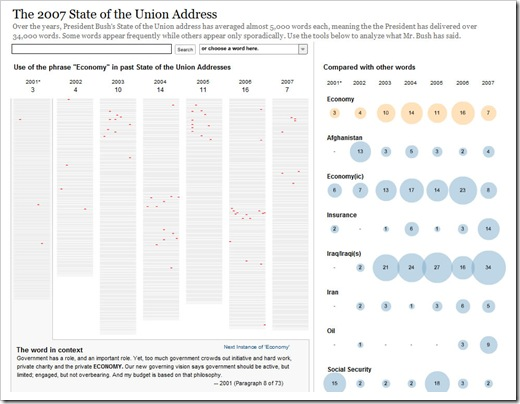
\includegraphics[width=1.0\textwidth]{plots/nytimesUnion.jpg} % requires the graphicx

(Left graph) The data is the text of the State of The Union Speeches from 2001 - 2007. x \& y positions of each word are mapped to the position of the word within the speech, paragraphs are separated by horizontal white lines.
Each word is represented by a small rectangle, which is colored red if selected, grey otherwise.  The plots are facetted on the x axis by year. The top of each graph is labelled by year. Beneath the label, the number of times the selected word appears is displayed.

(Right graph)  The data remains the text of the State of the Union speeches from 2001 - 2007, but now only a summary of the data is plotted: the number of times the selected word occurred in a speech. x and y positions are fixed for each summary, and the graph is facetted by year on the x axis and word on the y axis. The summaries are displayed with two layers: One layer of points with size proportional to frequency, and a second layer of text giving exact frequencies.

\section{How Class works - Components of Class}
\href{http://www.nytimes.com/packages/html/national/20050515\_CLASS\_GRAPHIC/index\_01.html}{http://www.nytimes.com/packages/html/national/20050515\_CLASS\_GRAPHIC/index\_01.html}\\

  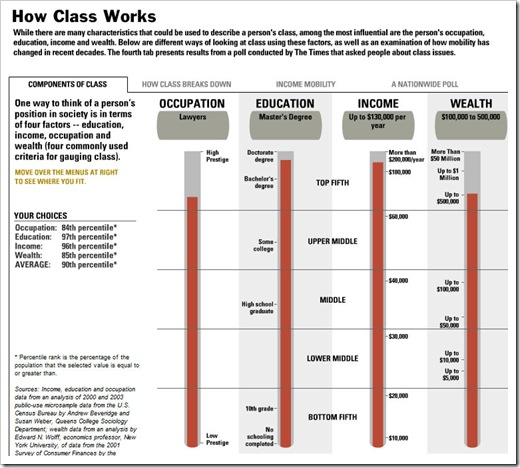
\includegraphics[width=1.0\textwidth]{plots/nytimesHowClassWorks.jpg} % requires the graphicx

The data is a collection of personal descriptors and the perceived "social worth" attached to each descriptor. x position remains constant. y position is mapped to the percentile of social worth represented by the selected value when compared to all values within the category. The graph is faceted on the x axis by category of descriptor: occupation, level of education, income, and accumulated wealth. A bottom layer uses gray rectangles to display the 100th percentile. A second layer displays Percentile with a slightly thinner red rectangle that extends from the bottom of the y axis to the value of the percentile. A third layer of horizontal lines divides the graphs into quintiles associated with different socioeconomic classes. And a fourth layer of text annotates various points of interest along the y axis of the four graphs.



\section{Is it Better to Buy or Rent?}
\href{http://www.nytimes.com/2007/04/10/business/2007\_BUYRENT\_GRAPHIC.html?\_r=1}{http://www.nytimes.com/2007/04/10/business/2007\_BUYRENT\_GRAPHIC.html?\_r=1}\\

  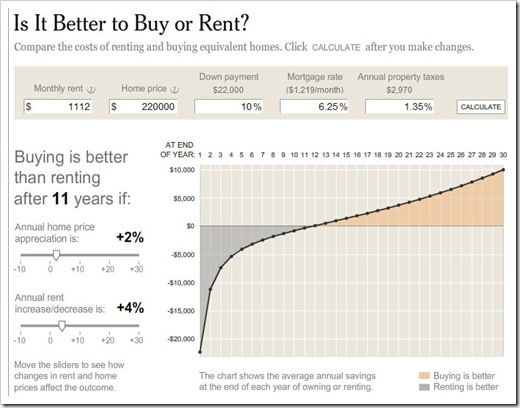
\includegraphics[width=1.0\textwidth]{plots/nytimesBuyOrRent.jpg} % requires the graphicx

The data is the amount of money that will be saved by buying a house by the number of years that the house will be owned. The interactive feature allows you to generate a new data set by customizing the values of variables, such as taxes and mortgage rates, that are used to calculate savings. y position is mapped to the savings that have accumulated from buying the house. x position is mapped to the number of years spent buying or renting the house. The savings at the end of a given number of years are represented by three layers: a layer of gray points, a layer with a gray line (that connects the points), and a layer that displays the area between the points and the line y = 0 with a fill color corresponding to whether the area is positive or negative. The x axis is annotated at the top of the plot instead of the bottom.



\section{The Ebb and Flow of Movies}
\href{http://www.nytimes.com/interactive/2008/02/23/movies/20080223\_REVENUE\_GRAPHIC.html}{http://www.nytimes.com/interactive/2008/02/23/movies/20080223\_REVENUE\_GRAPHIC.html}\\

  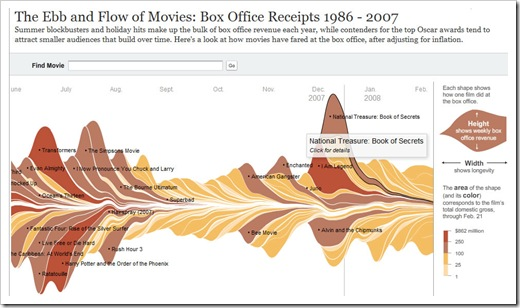
\includegraphics[width=1.0\textwidth]{plots/nytimesmoviebox.jpg} % requires the graphicx

The data is the weekly box office revenue of various movies recorded by date and movie. y position is mapped to weekly box office revenue. y position is mapped to the date with x limits set at January 1986 and February 2008. The weekly revenue is represented by a ribbon whose height corresponds to the weekly revenue and whose color corresponds to the total revenue earned by the movie (this is a statistical summary of the weekly data (a summation)). To avoid overplotting, the graph stacks ribbons on top of one another. A layer of vertical lines marks the beginning of each year. A layer of points marks particular movies. A layer of test labels which movies these points refer to. Legends appear to the right of the graph that explain the area scale and the color scale.

\section{Idaho Nominating Contest Results - Margin of Victory}
\href{http://politics.nytimes.com/election-guide/2008/results/states/ID.html}{http://politics.nytimes.com/election-guide/2008/results/states/ID.html}\\
Click "Margin of Victory"

  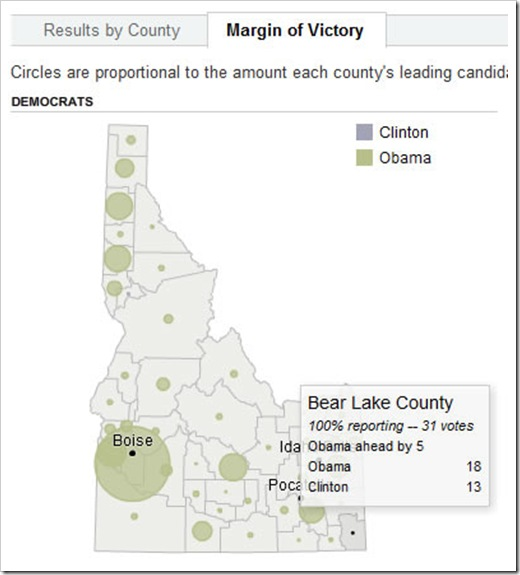
\includegraphics[width=1.0\textwidth]{plots/primary.jpg} % requires the graphicx


The data is the electoral results of the Idaho nominations. x and y positions are mapped to latitude and longitude. The margin of victory by county (a statistical summary of the data) is represented by a point. The points are plotted in the center of the counties that they correspond to. The size of the point is mapped to how large the margin is. The color of the point is mapped to who holds the lead. A legend in the top right corner displays the color scale. A map layer appears beneath the points that displays the county borders in the state of Idaho.  A layer of black points identifies cities of interest. A layer of black text identifies which city each black point corresponds to. The graph is facetted on the x axis by political party (Democrats and Republicans).

\section{How Different Groups Spend their Day}
\href{http://www.nytimes.com/interactive/2009/07/31/business/20080801-metrics-graphic.html}{http://www.nytimes.com/interactive/2009/07/31/business/20080801-metrics-graphic.html}\\

  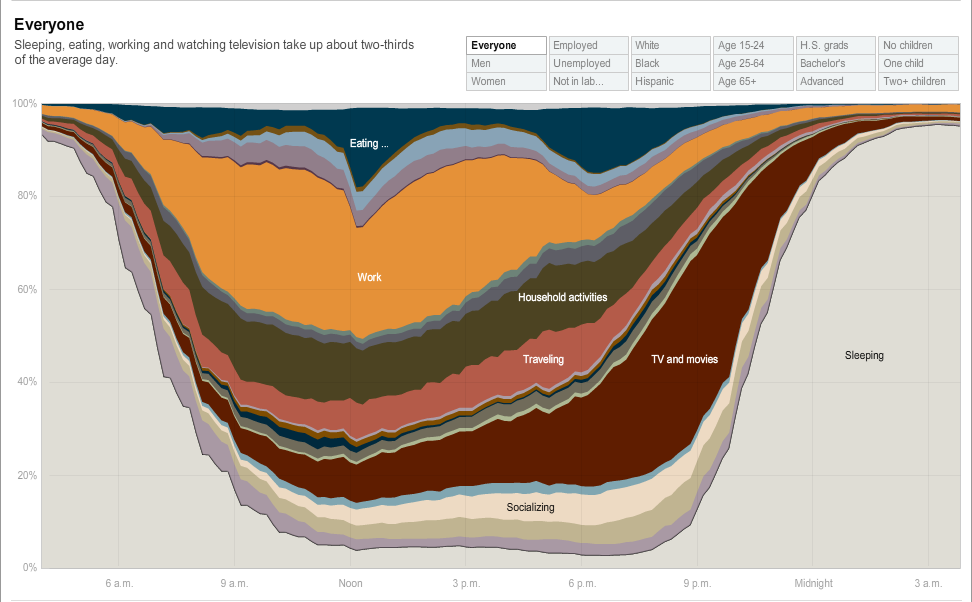
\includegraphics[width=1.0\textwidth]{plots/everyone.png} % requires the graphicx

The data is which of 21 activites respondents reported doing at each minute of the day. x position is time of the day. y position is the percentage of respondents doing the activity at that time (a summary from the data). The percentage is represented by a ribbon whose color corresponds to the activity. To avoid over plotting, the ribbons are offset in the "fill" manner (the total height is normalized at one, and the width of each ribbon shows the proportion of the total that it occupies). A layer of text objects identifies which activities the thickest ribbons correspond to.



\end{document}
